\chapter{Assignment \#3: Rankine Cycle, Enhanced Regeneration}
\label{ch:ass3}

\begin{fullwidth}
\newthought{Consider the } Rankine cycle depicted in the figure below:

\begin{figure}
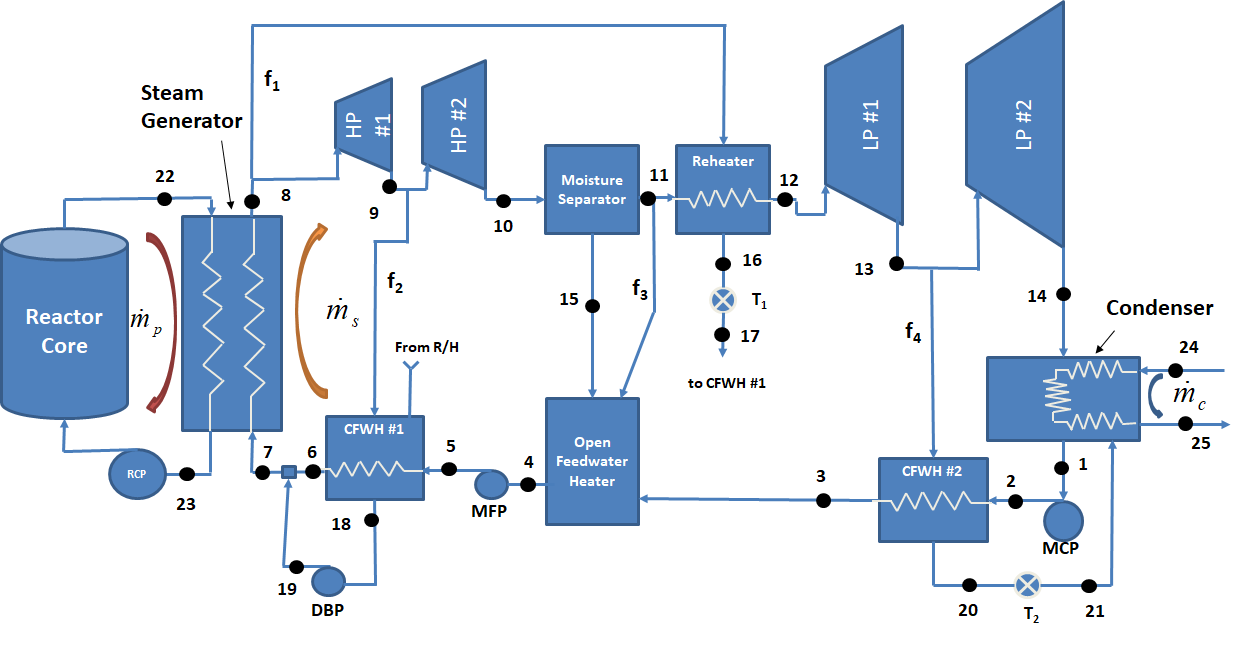
\includegraphics[width=12.0cm]{PowerCycleSchematic.png}
\caption{Power Cycle for Assignment \#3.}
\end{figure}

\begin{table}
\begin{tabular}{c | l || c | l}
\toprule
State Point & Notes & State Point & Notes \\
\hline
1 & P = 1.5 psia, x = 0.0 & 2 & P=164 psia \\
\hline
3 & T=T$_{\text{sat@ 62 psia}}$, P=164 psia & 4 & P = 164 psia\\
\hline
5 & P=838 psia, $\eta_{\text{MFP}} = 0.88$ & 6 & P = 838 psia, T=T$_{\text{sat @ 410 psia}}$ \\
\hline
7 & P = 838 psia & 8 & P=838 psia, x=1.0 \\
\hline
9 & P = 410 psia & 10 & P=164 psia \\
\hline
11 & P=164 psia & 12 & P=164 psia, T=490$^{\circ}$F \\
\hline
13 & P=62 psia & 14 & P=1.5 psia \\
\hline
15 & P=164 psia & 16 & P=838 psia, x=0.0 \\
\hline
17 & P=410 psia, isenthalpic expansion through T$_{1}$ & 18 & P=410 psia, x=0.0 \\
\hline
19 & P=838 psia & 20 & P=62 psia, x=0.0 \\
\hline
21 & P=1.5 psia, isenthalpic expansion through T$_{2}$ & 22 & P=2240 psia, T=610$^{\circ}F$ \\
\hline
23 & P=2240 psia, T=535$^{\circ}$F & 24 & P=14.7 psia, T=91$^{\circ}$F \\
\hline
25 & P=14.7 psia, T=115$^{\circ}$F & & \\
\hline
$\dot{m}_{p}$ & $113.5 \times 10^{6}$ lb$_{\text{m}}$/hr & Dead State & T$_{o}$=551$^{\circ}$R, P$_{o}$=14.7 psia \\
\bottomrule
\end{tabular}
\end{table}

\section{First Law Analysis}
\begin{enumerate}
\item Calculate pressure, temperature, enthalpy, entropy, quality, and specific flow exergy for each state point. [use USCS units throughout]

\vspace{1.0 cm}

\item Form energy-balance equations for CFWH\#1 and CFWH\#2.  Use \emph{fmincon} to solve for the flow fraction components of $f_1$, $f_2$, $f_3$, $f_4$, and the enthalpy at state point 7. [ flow fractions are unitless, $h_7$ is in BTU/lb$_\text{m}$]

\vspace{1.0cm}

\item Find the specific work for all pumps and turbines.[BTU/lb$_\text{m}$]

\vspace{1.0 cm}
\item Find the specific heat added in the SG and specific heat rejected in the condenser. [BTU/lb$_\text{m}$]

\vspace{1.0 cm}

\item Calculate the mass flow rate of steam from the steam generator $(\dot{m_{s}})$ and mass flow rate of condenser cooling water $(\dot{m_{c}})$.
\vspace{1.0cm}

\item Verify that $w_{\text{net}} = q_{\text{net}}$.

\vspace{1.0 cm}

\item What is the thermal efficiency for this cycle?

\end{enumerate}

\section{Second Law Analysis}

\begin{enumerate}[resume]
\item Calculate the total exergy transfer by work for the cycle. [BTU/hr]

\vspace{1.0cm}
\item Calculate the rate of exergy destruction in each component of the cycle. [BTU/hr]

\vspace{1.0cm}

\item Verify that the second law energy balance is satisfied:
$$\text{Exergy in - Exergy out = Exergy Destroyed + Exergy Transfer Through Work}$$

\vspace{1.0cm}

\item \textbf{\emph{Question for discussion:}} What components of the NSSS are most responsible for exergy destruction?  What design modifications would you consider to improve thermal efficiency?
\end{enumerate}

\end{fullwidth}
